
\documentclass{article}
\usepackage[spanish]{babel} %Definir idioma español
\usepackage[utf8]{inputenc} %Codificacion utf-8
\usepackage{amssymb, amsmath, amsbsy, wasysym}
\usepackage{multirow} % para tablas
\usepackage{graphicx}
\usepackage{listings}
\title{Tarea 1\\Control inteligente}
\author{Emmanuel Peto Gutiérrez}
\begin{document}
\maketitle

Se tiene un sistema con función de transferencia: $$G(s) = \frac{3000}{s^3 + 150s^2 + 1000s + 500}$$.

\section{Control tradicional}

Primero se diseñó un sistema con control tradicional, con los valores
\begin{itemize}
\item $k_p = 5$
\item $k_i = 0.5$
\item $k_d = 0.1$
\end{itemize}

con intervalo de tiempo de 0.1 s.

En la Figura \ref{tradicional_y} se muestra cómo cambia $y(k)$ respecto al tiempo y en la Figura \ref{tradicional_error} el error respecto al tiempo. El valor objetivo de $y(k)$ es 1 y se puede observar cómo su valor oscila entre 0 y 1.7 hasta que poco a poco alcanza el valor deseado de 1. En la gráfica de error se observa que éste se acerca al 0 hasta el segundo 5.

\begin{figure}
\center
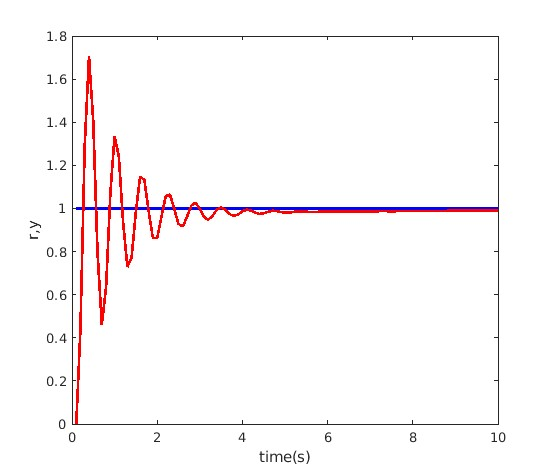
\includegraphics[scale=0.5]{trady.jpg}
\caption{Control tradicional: $y(k)$ respecto a $t$.}
\label{tradicional_y}
\end{figure}

\begin{figure}
\center
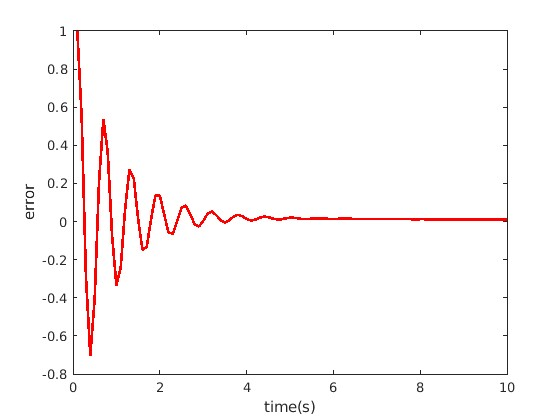
\includegraphics[scale=0.5]{trad_error.jpg}
\caption{Control tradicional: error respecto a $t$.}
\label{tradicional_error}
\end{figure}

El script de Matlab que se usó para el sistema de control tradicional fue el siguiente.

\begin{verbatim}
close all;
ts = 0.1;
sys = tf(3000,[1,150,1000,500]); %Planta
dsys=c2d(sys,ts,'z');
[num,den]=tfdata(dsys,'v');
u_1=0;u_2=0;u_3=0;u_4=0;
y_1=0;y_2=0;y_3=0;
ei=0;

kp=5;
ki=0.5;
kd=0.1;
sz = 100;

time = zeros(1,sz);
yd = zeros(1,sz);
y = zeros(1,sz);
error = zeros(1,sz);
derror = zeros(1,sz);
u = zeros(1,sz);

error_1=0;
for k=1:1:sz
    time(k) = k*ts;
    yd(k) = 1.0;
    y(k) = -den(2)*y_1 - den(3)*y_2 - den(4)*y_3 + num(2)*u_1 + num(3)*u_2 + num(4)*u_3;
    error(k) = yd(k)-y(k);
    derror(k) = error(k) - error_1;
    ei = ei + error(k)*ts;

    u(k)=kp*error(k)+kd*derror(k)/ts+ki*ei; %PID Controller
    u_4=u_3;u_3=u_2;u_2=u_1;u_1=u(k);
    y_3=y_2;y_2=y_1;y_1=y(k);
    error_1=error(k);
end
\end{verbatim}

\section{Control experto}

En el control experto se usaron los siguientes valores:

\begin{itemize}
\item $k_p = 0.5$
\item $k_i = 0.2$
\item $k_d = 0.05$
\end{itemize}

Las gráficas de $y(k)$ y error se muestran en las figuras \ref{experto_y} y \ref{experto_error}. En este caso se observa que el error disminuye rápidamente hasta acercarse al 0 en el segundo 2.

\begin{figure}
\center
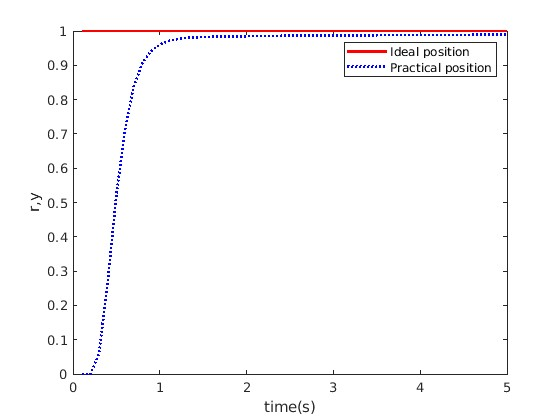
\includegraphics[scale=0.5]{expy.jpg}
\caption{Control experto: $y(k)$ respecto a $t$.}
\label{experto_y}
\end{figure}

\begin{figure}
\center
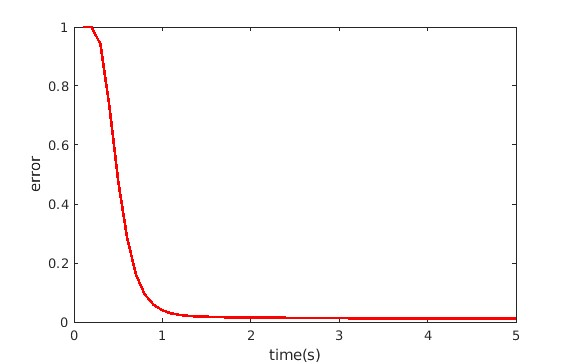
\includegraphics[scale=0.5]{exp_error.jpg}
\caption{Control experto: error respecto a $t$.}
\label{experto_error}
\end{figure}

El script del control experto es el siguiente:

\begin{verbatim}
close all;
ts=0.1;
sys = tf(3000,[1,150,1000,500]); %Planta
dsys=c2d(sys,ts,'z');
[num,den]=tfdata(dsys,'v');
u_1=0;u_2=0;u_3=0;u_4=0;
y_1=0;y_2=0;y_3=0;
ei=0;
error_1=0;error_2=0;derror_1=0;

kp = 0.5;
ki = 0.2;
kd = 0.05;

k1 = 1.95;
k2 = 0.45;
M1_1 = 0.8;
M1_2 = 0.6;
M1_3 = 0.4;
M1_4 = 0.01;
M2 = 0.08;
epsilon = 0.001;

sz = 50; %número de iteraciones
time = zeros(1,sz);
yd = zeros(1,sz);
y = zeros(1,sz);
error = zeros(1,sz);
derror = zeros(1,sz);
u = zeros(1,sz);

for k=1:1:sz
    time(k)=k*ts;
    yd(k)=1.0;
    % Linear model
    y(k) = -den(2)*y_1 - den(3)*y_2 - den(4)*y_3 + num(1)*u_1
    + num(2)*u_2 + num(3)*u_3 + num(4)*u_4;
    error(k)=yd(k)-y(k); % Calculating P
    derror(k)=error(k)-error_1; % Calculating D
    ei=ei+error(k)*ts; % Calculating I
    u(k)=kp*error(k) + (kd*derror(k))/ts + ki*ei; %tradicional
    
    % Expert control rule
    % Rule1:Unclosed control rule
    if abs(error(k)) > M1_1
        u(k) = 0.5;
    elseif abs(error(k)) > M1_2
        u(k) = 0.3;
    elseif abs(error(k)) > M1_3
        u(k) = 0.1;
    elseif abs(error(k)) > M1_4
        u(k) = 0.1;
    end

    % Rule 2
    if error(k)*derror(k)>0 || derror(k)==0
        if abs(error(k)) >= M2
            %control fuerte
            %u(k) = u_1 + k1*(kp*(error(k)-error_1)
            + ki*error(k) + kd*(error(k)-2*error_1+error_2));
            u(k) = u_1 + 1.6*kp*error(k);
        else
            %control débil
            %u(k) = u_1 + kp*(error(k)-error_1) + ki*error(k)
            + kd*(error(k)-2*error_1+error_2);
            u(k) = u_1 + 0.35*kp*error(k);
        end
    end

    % Rule 3
    if (error(k)*derror(k)<0 && derror(k)*derror_1>0) || (error(k)==0)
        u(k) = 1.65*u(k);
    end

    % Rule 4
    if error(k)*derror(k)<0 && derror(k)*derror_1<0
        if abs(error(k)) >= M2
            u(k)=u_1 + k1*kp*error(k);
        else
            u(k)=u_1 + k2*kp*error(k);
        end
    end

    % Rule5:Integration separation PI control
    if (abs(error(k)) <= epsilon)
        u(k)=0.4*error(k)+0.01*ei;
    end

    u_4=u_3;u_3=u_2;u_2=u_1;u_1=u(k);
    y_3=y_2;y_2=y_1;y_1=y(k);
    error_2=error_1;error_1=error(k);
    derror_1=derror(k);
end
\end{verbatim}

\end{document}

